\documentclass[11pt]{article}
\usepackage{fullpage,lipsum,amsmath,amsfonts,amssymb,graphicx, subcaption,enumitem,mathtools,float}
\font\titlefont=cmr12 at 20pt
\font\subtitlefont=cmr12 at 17pt

\title{%
  \titlefont{COMS W4701: Artificial Intelligence, Spring 2025} \\
\subtitlefont{Homework \#3}} %replace \# with number
\author{Peter Driscoll (pvd2112)} %replace with name & uni

\begin{document}
\maketitle

%Problem 1
\section*{Problem 1}

%Subsection 1.a
\subsection*{1.a)}
\begin{figure}[H]
\centering
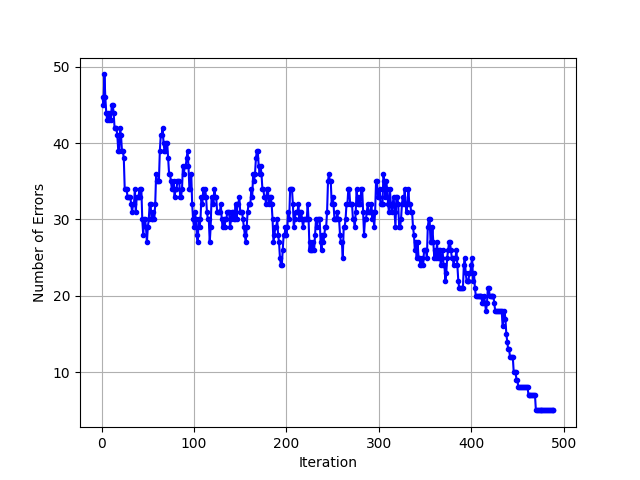
\includegraphics[width=0.7\textwidth]{images/Figure_1.jpg}
\vspace{1em}

\caption{Mini-Blackjack State Transition Diagram}
\label{fig:1}
\end{figure}

%Subsection 1.b
\subsection*{1.b)}
The optimal action for states 5 and 6 is the $stop$ action. The stop action at these states yields $V^*(\text{stop}) = 5$ and $V^*(\text{stop}) = 6$, respectively.
This is because the draw action from these states will always result in a sum greater than 6, which yields $V^*(\text{done}) = 0$.

\pagebreak

\begin{table}[h]
\centering
\renewcommand{\arraystretch}{1.5} % Increases row height for better readability
\caption{Optimal Actions and Values for Remaining States}
\label{tab:optimal_values}
\vspace{1em}

\begin{tabular}{c|l}
\hline
\textbf{State} & \textbf{Optimal Value Calculation} \\
\hline
4 &
$V(4) = \max \left\{  \frac{1}{3} \cdot V(6), 4 \right\}
\Rightarrow \max \left\{ 2 , 4  \right\}
\Rightarrow 4$ \\
\hline

3 &
$V(3) = \max \left\{  \frac{1}{3} \cdot (V(5) + V(6)), 3 \right\}
\Rightarrow \max \left\{ \frac{11}{3} , 3  \right\}
\Rightarrow \frac{11}{3}$ \\
\hline

2 &
$V(2) = \max \left\{  \frac{1}{3} \cdot (V(4) + V(5) + V(6)), 2 \right\}
\Rightarrow \max \left\{ 5 , 2  \right\}
\Rightarrow 5$ \\
\hline

0 &
$V(0) = \max \left\{ \frac{1}{3} V(2) + \frac{1}{3} V(3) + \frac{1}{3} V(4) , 0  \right\} \Rightarrow \frac{38}{9}$ \\
\hline
\end{tabular}
\end{table}

\vspace{1em}

\begin{table}[h]
\centering
\renewcommand{\arraystretch}{1.3} % Adjust row height for readability
\caption{Summary Optimal Actions and Values} % This caption will make it "Table 2"
\label{tab:summary_optimal_values} % You can reference it in the text with \ref{tab:optimal_values}
\[
\begin{array}{c|c|c}
  \text{State} & \pi^*_{t=1}(\text{state})
  & V^*(\text{state}) \\ \hline
  0 & \text{draw} & \frac{32}{9} \\
  2 & \text{draw} & 5 \\
  3 & \text{draw} & \frac{11}{3} \\
  4 & \text{stop} & 4 \\
  5 & \text{stop} & 5 \\
  6 & \text{stop} & 6
\end{array}
\]
\end{table}

Dynamic programming is not required for this problem because there is a chain of dependencies amongst the different states that obviates the need for
iterative value updates. Specifically, the states of 5 and 6 have trivial optimal values equal to their starting states, while state 4 only depends on
comparing its starting value to a reduced value of state 6, and so on and so forth for states 0, 2, and 3.

%Subsection 1.c
\subsection*{1.c)}

\begin{align*}
V^*(2) &\Rightarrow \text{ Need to find } \gamma \text{ s.t. } \\
& \Rightarrow \gamma \cdot \frac{11}{3} < 3 \\
&\Rightarrow \gamma \leq \frac{9}{11}
\end{align*}

\vspace{1em}

\begin{align*}
V^*(3) &\Rightarrow \text{ Need to find } \gamma \text{ s.t. } \\
&\Rightarrow \gamma \cdot 5 < 3 \\
&\Rightarrow \gamma \leq \frac{2}{5}
\end{align*}

Thus,
\[
\gamma = \min\left\{\frac{2}{5}, \frac{9}{11}\right\} = \frac{2}{5}
\]

Substituting \(\gamma = \frac{2}{5}\) into the computation of \(V^*(3,2,0)\) results in the following:

\begin{table}[h]
\centering
\renewcommand{\arraystretch}{1.5} % Increases row height for better readability
\caption{$\gamma$-min Optimal Actions and Values for Remaining States}
\label{tab:lambda_min_optimal_values}
\vspace{1em}

\begin{tabular}{c|l}
\hline
\textbf{State} & \textbf{Optimal Value Calculation} \\
\hline

3 &
$V_1(3) = \max \left\{ \frac{2}{5} \cdot \frac{5+6}{3}, 3 \right\}
\Rightarrow \max \left\{ 22/15 , 3  \right\}
\Rightarrow 3$ \\
\hline

2 &
$V_1(2) = \max \left\{ \frac{2}{5} \cdot \frac{4+5+6}{3}, 2 \right\}
\Rightarrow \max \left\{ 2 , 2  \right\}
\Rightarrow 2$ \\

\hline

0 &
$V_1(0) = \max \left\{ \frac{2}{5} \cdot (V(2) + V(3) +  V(4)) , 0  \right\} \Rightarrow \frac{6}{5}$ \\
\hline
\end{tabular}
\end{table}

A lower discount factor \(\gamma\) reduces the values of states 0, 2 and 3 because these states have lower starting values and depend on the draw action,
to reach their optimal terminal value, making them more sensitive to a decrease in $\gamma$.
In contrast, states 4, 5, and 6 have such high starting values that their optimal values are secured by choosing the \textit{done} action at the outset,
making them fully insensitive to downward changes in $\gamma$.

%Problem 2
\section*{Problem 2}
\subsection*{2.a)}
The $\pi^*$ and $V^*$ for the updated mini-blackjack game will now bias exclusively toward drawing cards until reaching the state of 6 and
then stopping, thus the $\pi^*$ will return the draw actions for states less than 6, and the $V^*$ will be 6 for all states.

\subsection*{2.b)}

\begin{align*}
  V_{i+1}(0) &= \max\Biggl\{
    T(0,\text{stop},\text{done})\Bigl[R(0,\text{stop},\text{done}) + 0.9\,V_i(\text{done})\Bigr], \\
    &\quad\; T(0,\text{draw},2)\Bigl[R(0,\text{draw},2) + 0.9\,V_i(2)\Bigr] \\
    &\quad\; +\; T(0,\text{draw},3)\Bigl[R(0,\text{draw},3) + 0.9\,V_i(3)\Bigr] \\
    &\quad\; +\; T(0,\text{draw},4)\Bigl[R(0,\text{draw},4) + 0.9\,V_i(4)\Bigr]
  \Biggr\}, \\[1ex]
  V_{i+1}(2) &= \max\Biggl\{
    T(2,\text{stop},\text{done})\Bigl[R(2,\text{stop},\text{done}) + 0.9\,V_i(\text{done})\Bigr], \\
    &\quad\; T(2,\text{draw},4)\Bigl[R(2,\text{draw},4) + 0.9\,V_i(4)\Bigr] \\
    &\quad\; +\; T(2,\text{draw},5)\Bigl[R(2,\text{draw},5) + 0.9\,V_i(5)\Bigr] \\
    &\quad\; +\; T(2,\text{draw},6)\Bigl[R(2,\text{draw},6) + 0.9\,V_i(6)\Bigr]
  \Biggr\}, \\[1ex]
  V_{i+1}(3) &= \max\Biggl\{
    T(3,\text{stop},\text{done})\Bigl[R(3,\text{stop},\text{done}) + 0.9\,V_i(\text{done})\Bigr], \\
    &\quad\; T(3,\text{draw},5)\Bigl[R(3,\text{draw},5) + 0.9\,V_i(5)\Bigr] \\
    &\quad\; +\; T(3,\text{draw},6)\Bigl[R(3,\text{draw},6) + 0.9\,V_i(6)\Bigr] \\
    &\quad\; +\; T(3,\text{draw},0)\Bigl[R(3,\text{draw},0) + 0.9\,V_i(0)\Bigr]
  \Biggr\}, \\[1ex]
  V_{i+1}(4) &= \max\Biggl\{
    T(4,\text{stop},\text{done})\Bigl[R(4,\text{stop},\text{done}) + 0.9\,V_i(\text{done})\Bigr], \\
    &\quad\; T(4,\text{draw},6)\Bigl[R(4,\text{draw},6) + 0.9\,V_i(6)\Bigr] \\
    &\quad\; +\; T(4,\text{draw},0)\Bigl[R(4,\text{draw},0) + 0.9\,V_i(0)\Bigr] \\
    &\quad\; +\; T(4,\text{draw},0)\Bigl[R(4,\text{draw},0) + 0.9\,V_i(0)\Bigr]
  \Biggr\}, \\[1ex]
  V_{i+1}(5) &= \max\Bigl\{
    T(5,\text{stop},\text{done})\Bigl[R(5,\text{stop},\text{done}) + 0.9\,V_i(\text{done})\Bigr],\;
    T(5,\text{draw},0)\Bigl[R(5,\text{draw},0) + 0.9\,V_i(0)\Bigr]
  \Bigr\}, \\[1ex]
  V_{i+1}(6) &= \max\Bigl\{
    T(6,\text{stop},\text{done})\Bigl[R(6,\text{stop},\text{done}) + 0.9\,V_i(\text{done})\Bigr],\;
    T(6,\text{draw},0)\Bigl[R(6,\text{draw},0) + 0.9\,V_i(0)\Bigr]
  \Bigr\}.
\end{align*}
\subsection*{2.c)}

\paragraph{Iteration 1 (\(V_1\))}
\[
V_1(0)
= \max\Bigl\{
0,\;
\tfrac{1}{3}\bigl(0 + 0\bigr)
+ \tfrac{1}{3}\bigl(0 + 0\bigr)
+ \tfrac{1}{3}\bigl(0 + 0\bigr)
\Bigr\}
= 0
\]

\[
V_1(2)
= \max\Bigl\{
2,\;
\tfrac{1}{3}\bigl(0 + 0\bigr)
+ \tfrac{1}{3}\bigl(0 + 0\bigr)
+ \tfrac{1}{3}\bigl(0 + 0\bigr)
\Bigr\}
= 2
\]

\[
V_1(3)
= \max\Bigl\{
3,\;
\tfrac{1}{3}(0)
\Bigr\}
\;\;=\;\;3
\]

\[
V_1(4)
= \max\Bigl\{
4,\;
\tfrac{1}{3}(0)
\Bigr\}
\;\;=\;\;4
\]

\[
V_1(5) \;=\; 5
\]

\[
V_1(6) \;=\; 6
\]

\paragraph{Iteration 2 (\(V_2\))}

\[
V_2(0)
= \max\Bigl\{
0,\;
\tfrac{1}{3}\bigl(0 + 0.9 \times 2\bigr)
+ \tfrac{1}{3}\bigl(0 + 0.9 \times 6\bigr)
+ \tfrac{1}{3}\bigl(0 + 0.9 \times 3\bigr)
\Bigr\}
\;=\;
\frac{9}{2}
\;=\;
4.5
\]

\[
V_2(2)
= \max\Bigl\{
2,\;
\tfrac{1}{3}\bigl(0 + 0.9 \times 5\bigr)
+ \tfrac{1}{3}\bigl(0 + 0.9 \times 6\bigr)
+ \tfrac{1}{3}\bigl(0 + 0.9 \times V_1(done)\bigr)
\Bigr\}
\;=\;\tfrac{9}{2}
\]

\[
V_2(3)
= \max\Bigl\{
3,\;
\tfrac{1}{3}\bigl(0 + 0.9 \times 5\bigr)
+ \tfrac{1}{3}\bigl(0 + 0.9 \times 6\bigr)
+ \tfrac{1}{3}\bigl(0 + 0.9 \times V_1(done)\bigr)
\Bigr\}
\;=\;
\frac{33}{10}
\;=\;
3.3
\]

\[
V_2(4)
= \max\Bigl\{
4,\;
\tfrac{1}{3}\bigl(0 + 0.9 \times 6\bigr)
+ \tfrac{2}{3}\bigl(0 + 0.9 \times V_1(done)\bigr)
\Bigr\}
\;=\;
\frac{33}{10}
\;=\;
3.3
\]

\[
V_2(5)
= \max\Bigl\{
5,\;
\tfrac{3}{3}\bigl(0 + 0.9 \times V_1(done)\bigr)
\Bigr\}
\;=\;
5
\]

\[
V_2(6)
= \max\Bigl\{
6,\;
\tfrac{3}{3}\bigl(0 + 0.9 \times V_1(done)\bigr)
\Bigr\}
\;=\;
6
\]
\subsection*{2.d)}
The convergence of value iteration is determined by the value of $\gamma$. Each update of V(s) shrinks the gap between $V^*(s) \text{ and } V(s)$ by
a factor of $\gamma$. Thus, reducing $\gamma$ to 0.5 will exponentially reduce the amount of iterations necessary to converge under the threshold.
I would expect the $\pi(\gamma = 0.9)$ to incur more draw actions because optimal value will be weighted more heavily toward future values, which
would retain more of their value in successive future iterations due to the higher $\gamma$.

\newpage
%Problem 3
\section*{Problem 3}
\subsection*{3.a)}
\paragraph{Episode 1:}
\[
V(0) = V(2) = V(4) = 0
\]

\paragraph{Episode 2:}
\[
V(0) = V(3) = 0
\]

\paragraph{Episode 3:}
\[
V(2) = \gamma^2(5) = 5
\quad\text{and}\quad
V(5) = \gamma^2(5) = 5.
\]
\[
V(2) = \frac{0 + 5}{2} = 2.5
\]

\paragraph{Episode 4:}
\[
V(3) = \gamma^2(5) = 5
\quad\text{and}\quad
V(5) = \gamma^2(5) = 5.
\]
\[
V(3) = \frac{0 + 5}{2} = 2.5
\]

\paragraph{Episode 5:}
\[
V(4) = 6
\quad\text{and}\quad
V(6) = 6.
\]
\[
V(4) = \frac{0 + 6}{2} = 3
\]

The order in which the episodes are observed does not affect the estimated state values. This is because Monte-Carlo prediction computes the value of
each state by averaging the rewards of each episode in which the state was visited. Because computing a simple average is a commutative operation, order
of the episodes does not impact the final estimated value of the states.

\subsection*{3.b)}

\paragraph{After Episode 3}
\[
V(0) = \frac{0 + 0 + 5}{3} = \frac{5}{3},\quad
V(2) = \frac{0 + 5}{2} = 2.5,\quad
V(5) = \frac{5}{1} = 5.
\]

\paragraph{After Episode 4}
\[
V(0) = \frac{0 + 0 + 5 + 5}{4} = \frac{10}{4} = 2.5,\quad
V(3) = \frac{0 + 5}{2} = 2.5,\quad
V(5) = \frac{5 + 5}{2} = 5.
\]

\paragraph{After Episode 5 (Final)}
\[
V(0) = \frac{0 + 0 + 5 + 5 + 6}{5} = 3.2,\quad
V(4) = \frac{0 + 6}{2} = 3.0,\quad
V(6) = \frac{6}{1} = 6.
\]
(States $2$, $3$, and $5$ do not appear in Episode 5, so their values remain $2.5$, $2.5$, and $5$, respectively.)

\paragraph*{Final Values}
\[
\boxed{
  V(0) = 3.2,\quad
  V(2) = 2.5,\quad
  V(3) = 2.5,\quad
  V(4) = 3.0,\quad
  V(5) = 5.0,\quad
  V(6) = 6.0.
}
\]
These are the Monte Carlo estimates of the state values after processing all five episodes.

\begin{flushleft}
  In TD learning the order in which the episodes are observed does affect the estimated state values.
  This is because TD learning updates states incrementally using the current estimate of the successor state, thus, the value of a state
  will immidiately impact the value of the succesor state, as determined by their relative order.
\end{flushleft}

\subsection*{3.c)}
The Q values learned by SARSA and Q-learning can differ in states where the behavior policy may sometimes select suboptimal actions.
This divergence arises because of the way the two algorithms update their Q values. Q-learning is an off-policy method.
It updates the Q value using the maximum possible Q value in the next state, that is,
it always uses the action that maximizes the expected return (according to the target policy).
Therefore, even if the behavior policy explores, Q-learning’s updates always assume that the best action is taken next.

SARSA is an on-policy method. It updates the Q value using the actual action taken by the behavior policy, which might sometimes be suboptimal due to
exploration, for example, an $\epsilon$-greedy policy might select a non-optimal action.

For example, in state 2, suppose the optimal action is to “draw”, which yields the optimal expected value of 5 rather than “stop”, which yields a suboptimal
expected return of 2. Q-learning will update state 2 using the Q value corresponding to “draw” (i.e., the maximum return), whereas SARSA might occasionally
update state 2 using the return for “stop” if the behavior policy happens to select that action. This difference leads SARSA to sometimes generate
lower Q values for states 2, 3 and 4, whose optimal values depend on taking a sequence of optimal actions.

\newpage
\section*{Problem 4}

\subsection*{4.a)}

% Discussion of the $\epsilon$-greedy strategy:
For the $\epsilon$-greedy method, Figure~\ref{fig:epsilon} illustrates that setting $\epsilon = 0.1$ performs best over the long term,
favoring less exploration. However, in shorter time frames, a higher $\epsilon$ is necessary to ensure that all $k$ arms are sufficiently tested.

\begin{figure}[htbp]
\centering
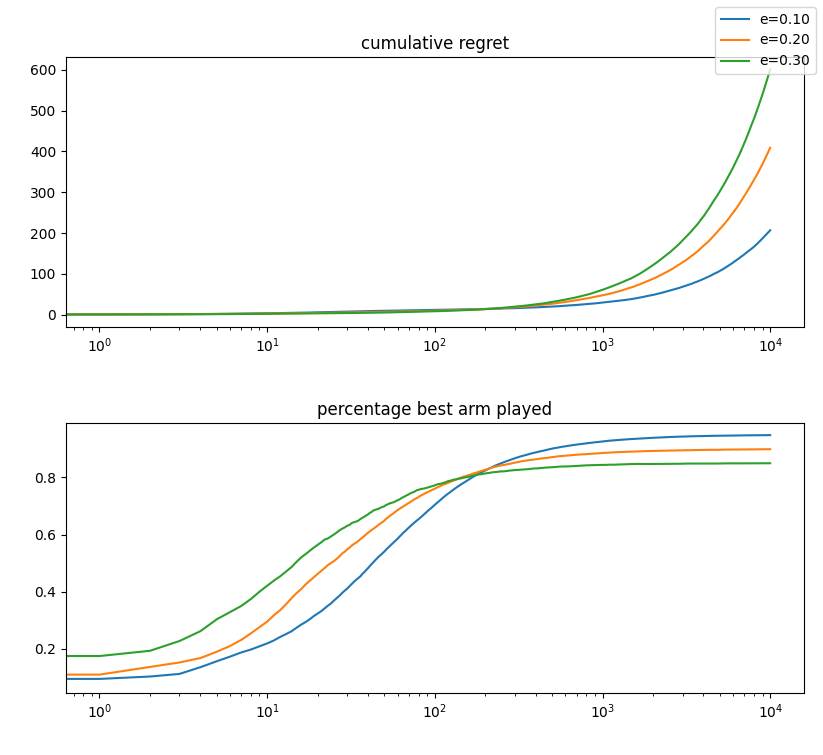
\includegraphics[width=0.8\textwidth]{images/Figure_2.png}
\caption{Performance of $\epsilon$-greedy with different values of $\epsilon$. Long-term performance is best with $\epsilon = 0.1$,
though higher values may be beneficial for early exploration.}
\label{fig:epsilon}
\end{figure}

\newpage

% Discussion of the UCB strategy:
In contrast, Figure~\ref{fig:ucb} demonstrates the UCB approach where the exploration parameter $c$ scales the exploration rate.
Here, setting $c = 0.3$ yields the best long-term performance, outperforming the $\epsilon$-greedy strategy significantly.

\begin{figure}[htbp]
\centering
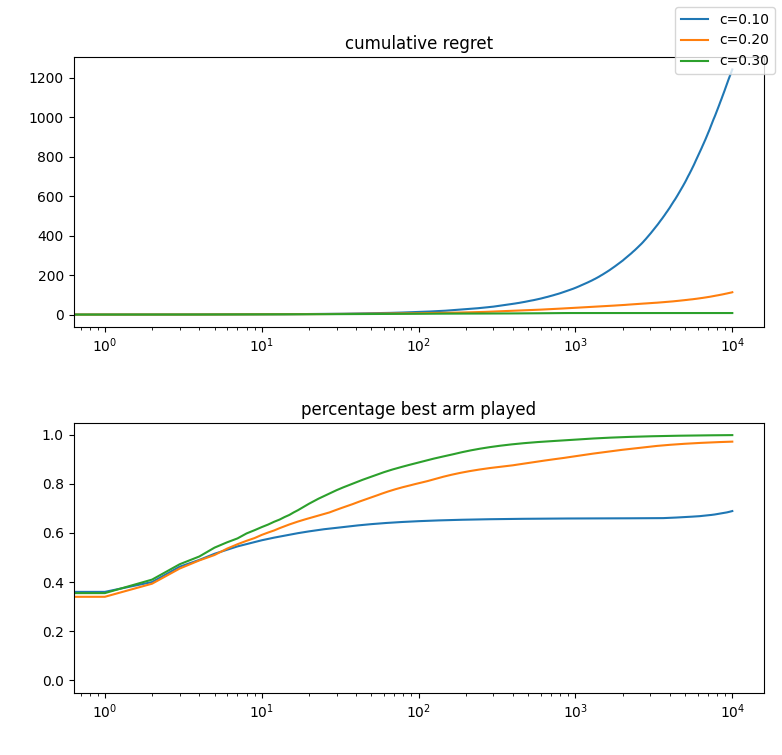
\includegraphics[width=0.8\textwidth]{images/Figure_3.png}
\caption{Performance of UCB with varying values of $c$. The best long-term performance is achieved when $c = 0.3$.}
\label{fig:ucb}
\end{figure}

\paragraph{}
Additionally, from a theoretical standpoint, the cumulative regret of $\epsilon$-greedy often grows \emph{linearly} in $T$,
whereas UCB methods achieve regret on the order of $\log T$. On the log-scale x-axis, linear growth appears almost
``exponential,'' while near-logarithmic growth appears roughly linear. This explains why, over large time horizons,
UCB typically outperforms $\epsilon$-greedy in terms of cumulative regret.

\newpage
\subsection*{4.b)}
% Discussion of the $\epsilon$-greedy strategy for more difficult bandit:
For the updated $\bigtriangleup$k values, the $\epsilon$-greedy method, Figure~\ref{fig:epsilon} illustrates that setting $\epsilon = 0.1$ still performs best over the long term,
favoring less exploration. However, the lower $\bigtriangleup$k makes the optimal arm more difficult to locate, necessitating a longer time to maximize frequency of
the best arm to 1.

\begin{figure}[htbp]
\centering
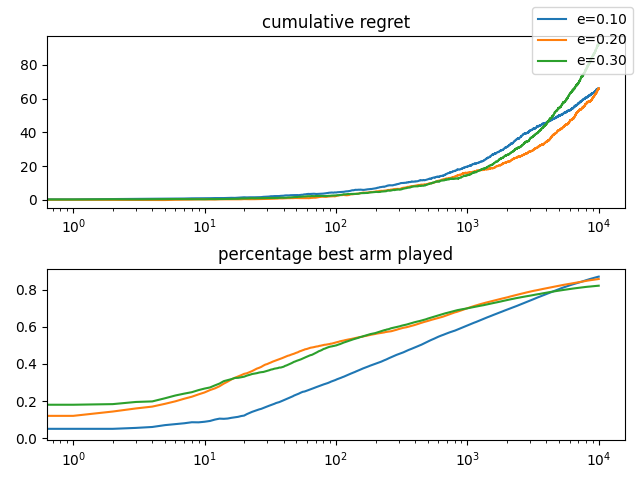
\includegraphics[width=0.8\textwidth]{images/Figure_4.png}
\caption{Performance of $\epsilon$-greedy with different values of $\epsilon$. Long-term performance is best with $\epsilon = 0.1$,
though higher values may be beneficial for early exploration.}
\label{fig:epsilon_hard}
\end{figure}

\newpage
% Discussion of the UCB strategy for more difficult bandit:
In contrast, Figure~\ref{fig:ucb} demonstrates the UCB approach where the exploration parameter $c$ scales the exploration rate.
Here, setting $c = 0.3$ still yields the best long-term performance, outperforming the $\epsilon$-greedy strategy by a much larger margin under the
lower $\bigtriangleup$k parameter. This indicates UCB is less sensitive to changes in $\bigtriangleup$k, likely stemming from the advantages inherent to UCB.
Namely, because k = 2, UCB is able to quickly hone in on the optimal arm using its more targeted exploration and under proper tuning (c = 0.1) its regret
grows $O(\log(N))$ better than $\epsilon$-greedy.

\begin{figure}[htbp]
\centering
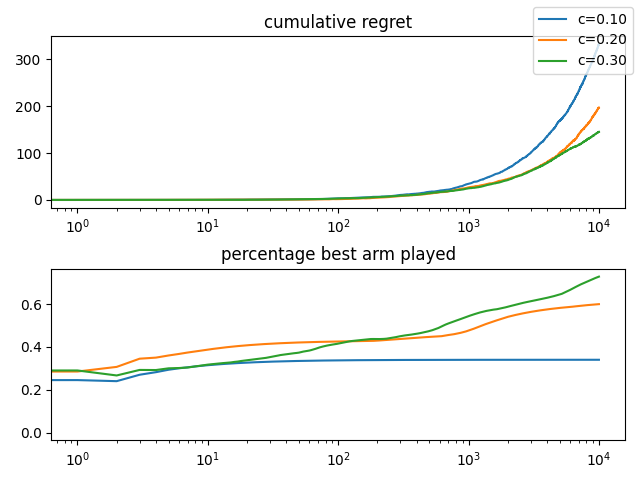
\includegraphics[width=0.8\textwidth]{images/Figure_5.png}
\caption{Performance of UCB with varying values of $c$. The best long-term performance is achieved when $c = 0.3$.}
\label{fig:ucb_hard}
\end{figure}

\newpage
\subsection*{4.c)}
% Discussion of the $\epsilon$-greedy strategy for more difficult bandit:
For the updated $\bigtriangleup k$ values, the $\epsilon$-greedy method, Figure~\ref{fig:epsilon_four_k} illustrates the difficulty that the $\epsilon$-greedy method
has in finding the optimal arm. The reason for this is twofold: doubling the number of arms increases the difficulty for the algorithm to find the optimal arm,
while increasing the range of reward variance amongst the arms increases the expected regret of having to explore suboptimal arms for a longer period of time.
This explains why the performance of the algorithm is the worst under $\epsilon = 0.3$, as the expected regret is maximized due to the increased selection
of arms with a high $\bigtriangleup k$. Moreover, since $\epsilon$-greedy continues to select random actions with a fixed probability,
its cumulative regret grows roughly linearly with time, exacerbating the penalty from repeatedly exploring inferior arms.

\begin{figure}[htbp]
\centering
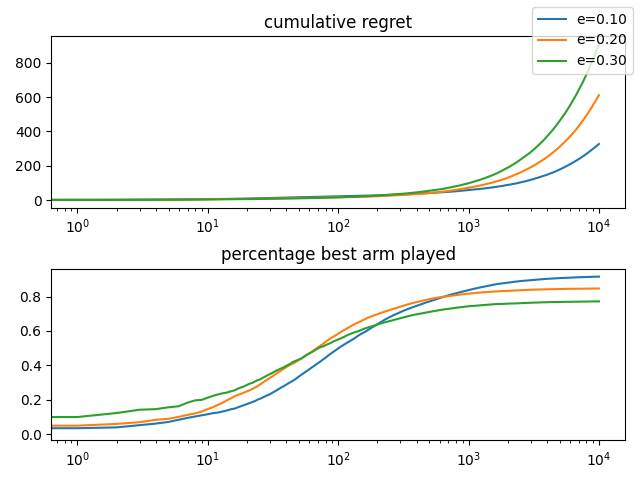
\includegraphics[width=0.8\textwidth]{images/Figure_6.png}
\caption{Performance of $\epsilon$-greedy with different values of $\epsilon$. Long-term performance is best with $\epsilon = 0.1$, though higher values may be beneficial for early exploration.}
\label{fig:epsilon_four_k}
\end{figure}

\newpage
% Discussion of the UCB strategy for more difficult bandit:
In contrast, Figure~\ref{fig:ucb_four_k} demonstrates that UCB has a much greater variance in performance compared to $\epsilon$-greedy when the number of arms is increased to 4.
However, when $c$ is properly chosen, the algorithm performs similarly in terms of the percentage of best arm selections,
yet it exhibits a significantly lower cumulative regret. This behavior owes to the fact that while both algorithms take more time to find the optimal arm,
UCB is able to iteratively hone in on the best arm by exploring those with values closer to the optimum rather than exploring uniformly at random.
Furthermore, UCB’s directed exploration typically results in a sublinear (often logarithmic) growth in cumulative regret, in contrast to the
linear regret growth inherent to $\epsilon$-greedy with fixed $\epsilon$.

\begin{figure}[htbp]
\centering
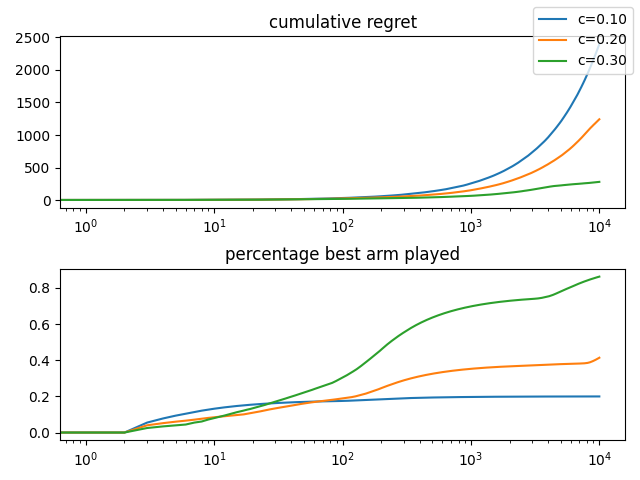
\includegraphics[width=0.8\textwidth]{images/Figure_7.png}
\caption{Performance of UCB with varying values of $c$. The best long-term performance is achieved when $c = 0.3$.}
\label{fig:ucb_four_k}
\end{figure}

\section*{Problem 5}
\subsection*{5.a)}

Increasing $\gamma$ to 0.9 makes the agent value future rewards more, leading to a higher 100-step average velocity (about 0.41 versus 0.16). Lowering $\gamma$
to 0.7 makes the agent more short-sighted, reducing the average velocity to around 0.11. Note that $\gamma$ affects how future rewards are weighted—not
the exploration rate.

\subsection*{5.b)}
After the robot has learned the optimal policy, increasing $\epsilon$ increases the avg velocity of the robot by around 20 percent, and decreasing $\epsilon$ has the opposite effect, reducing the average velocity by around 30 percent.

\subsection*{5.c)}
With $\alpha$ = 0.8 the robot averages about 3400 steps to cross, but lowering $\alpha$ to 0.1 increases the average to roughly 6000 steps. This shows that a higher learning rate speeds up Q-value convergence and reduces training time.
\end{document}

